\documentclass[a4paper]{article}
\usepackage[utf8]{inputenc}
\usepackage[russian,english]{babel}
\usepackage[T2A]{fontenc}
\usepackage[left=10mm, top=20mm, right=18mm, bottom=15mm, footskip=10mm]{geometry}
\usepackage{indentfirst}
\usepackage{amsmath,amsfonts,amssymb,amsthm,mathtools}
\usepackage[italicdiff]{physics}
\usepackage{graphicx}
\graphicspath{{images/}}
\DeclareGraphicsExtensions{.pdf,.png,.jpg}
\usepackage{wrapfig}

\usepackage{caption}
\captionsetup[figure]{name=Рисунок}
\captionsetup[table]{name=Таблица}
  
\title{\underline{Отчет о выполненой лабораторной работе 1.1.6}}
\author{Антон Хмельницкий, Б01-306}
\date{03.10.20}

\begin{document}

\maketitle


\begin{center}
\textbf{\Large Изучение электронного осциллографа}
\end{center}


\section{Аннотация}
\underline{Цель работы:} ознакомиться с устройством и органами управления электронного и/или цифрового осциллографа; научиться измерять амплитуды и частоты произвольных сигналов; изучить основные характеристики осциллографа и их влияние на искажение сигналов.

\underline{В работе используются}: осциллограф (электронный и/или цифровой), генераторы электрических сигналов, соединительные кабели.

\section{Теоретическая сведения}
Осциллограф — регистрирующий прибор, в котором исследуемый электрический сигнал (напряжение) преобразуется в видимый на экране график изменения величины сигнала во времени. Осциллографы широко используются в физическом эксперименте для регистрации изменения во времени любых физических величин, которые могут быть преобразованы в электрические сигналы.

В современных лабораториях используются электронно-лучевые (аналоговые) и цифровые осциллографы. В электронно-лучевом осциллографе входной сигнал подаётся на отклоняющие конденсаторные пластины, вызывающие пропорциональное отклонение пучка электронов, попадающих на люминофор электронно-лучевой трубки. В цифровых приборах аналоговый сигнал оцифровывается с помощью аналогово-цифрового преобразователя (АЦП), который сохраняется в памяти и затем отображается дисплее. Современные цифровые приборы обладают рядом несомненных преимуществ, таких как возможность записи сигнала, математической обработки, многоканальная регистрация и т.д. При этом их основные характеристики даже у относительно недорогих моделей практически не уступают аналоговым (а у профессиональных моделей — превосходят), поэтому цифровые осциллографы постепенно вытесняют аналоговые.


Основой осциллографа является электроннная лучевая трубка. Устройство электронной лучевой трубки осциллографа:

\begin{wrapfigure}{R}{.5\textwidth}
\centering
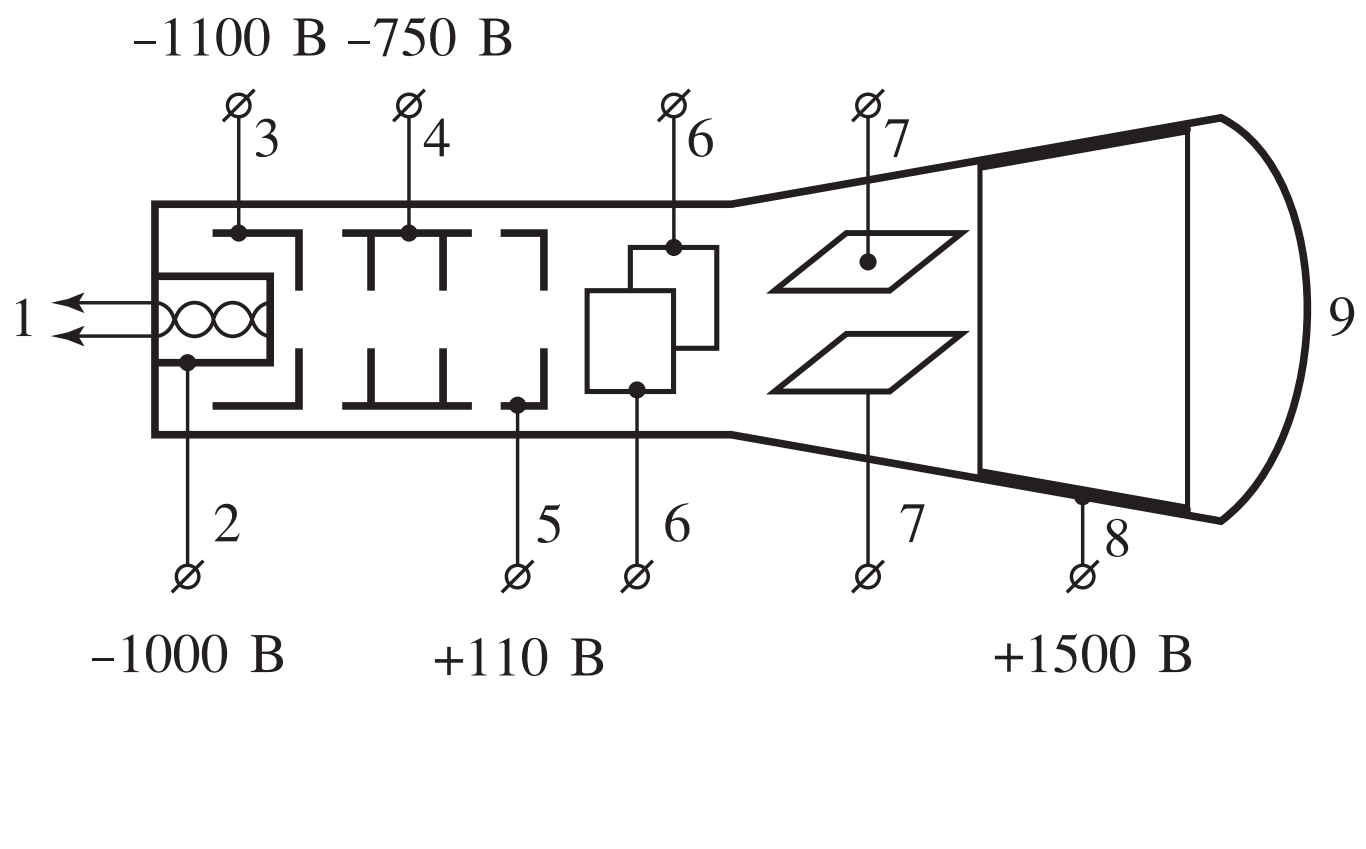
\includegraphics[width=0.4\textwidth]{1.png}
\caption{Электронно лучевая трубка}
\end{wrapfigure}

Здесь $1$ -- подогреватель катода, $2$ -- катод, $3$ -- модулятор, $4$ -- первый (фокусирующий)
анод, $5$ -- второй (ускоряющий) анод, $6$ и $7$ -- горизонтально и вертикально отклоняющие
пластины, $8$ -- третий (ускоряющий) анод, $9$ -- экран.

Электронный пучок формируется системой электродов, называемой "электронной пушкой": катод с нагревателем, модулятор, фокусирующий и ускоряющий аноды. Яркость изображения на экране осциллографа регулируется напряжением на модуляторе (изменяется ручкой "INTEN"), фокус изображения зависит от потенциала первого анода, который можно менять ручкой "FOCUS".

На пути пучка электронов находятся 2 конденстора, электрическое поле в которых взаимно ортогонально, чтобы отклонять пучок в двух взаимных направлениях декартовой системы координат. Регулируя напряжения на конденсаторах, можно определить положения пучка электронов на экране.

\begin{figure}[t]
    \centering
    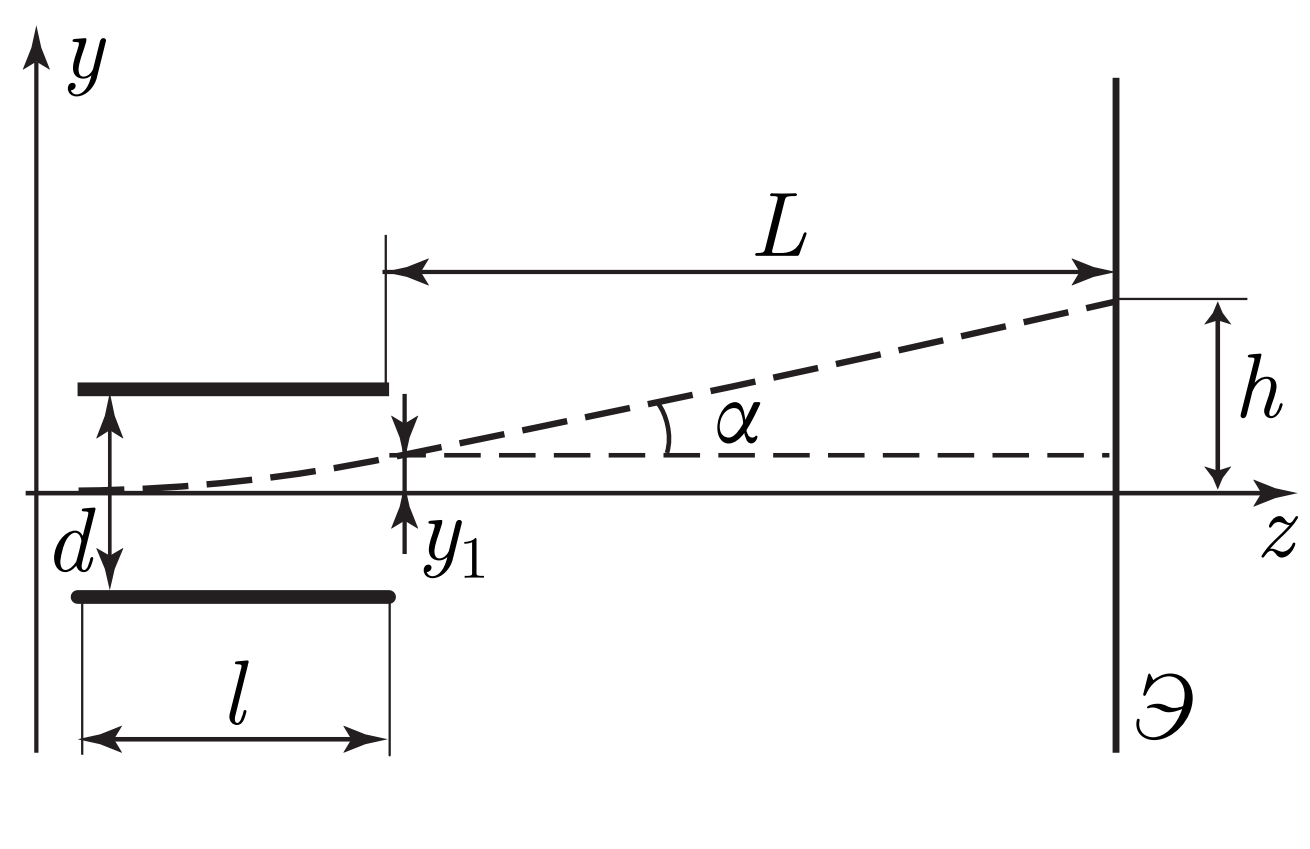
\includegraphics[width=0.4\textwidth]{2.png}
    \caption{Отклонения луча в электрическом поле пластин}
\end{figure}

Рассматривая движение пучка в электрических полях пластин можно вывести смещение $h$ электронного пятна на экране осциллографа: 
\[h_{y} =\frac{l(\frac{l}{2} + L)}{2dU_{a}}\cdot U_y \text{,  где $l$ - длина пластин, $L$ - расстояние от середины пластин до экрана, $d$ - расстояние между пластинами, $U_{a}$ - ускоряющее напряжение на втором аноде, $U_{y}$ - напряжение между пластинами.}\]

Чувствительность ЭЛТ к напряжению: 
\[K_{y} =\frac{2dU_{a}}{l(\frac{l}{2} + L)} \text{,  где $l$ - длина пластин, $L$ - расстояние от середины пластин до экрана, $d$ - расстояние между пластинами.}\]
Обе формулы применимы тогда, когда за время пролёта пучка \textit{переменное напряжение} на конденсаторах \textit{практически не меняется}. В итоге получается, что смещение частицы в выбранном направлении прямо пропорционально напряжению на конденсаторе.Таким образом, положение электронного пучка на экране осциллографа будет пропорционально мгновенному значению напряжения согласно выражению.

Итак, в рабочем режиме координаты $x$ и $y$ точки попадания электронного луча на экран (относительно его центра) пропорциональны мгновенным значениям напряжений $Ux(t)$ и $Uy(t)$, подаваемых на горизонтально и вертикально отклоняющие пластины. Ясно, что отклонение луча должно быть, во-первых, заметным и, во-вторых, не выходить за пределы экрана. Поэтому, чтобы иметь возможность исследовать сигналы в широком диапазоне амплитуд, подаваемые на пластины сигналы нужно предварительно усиливать или ослаблять. Для усиления слабых сигналов в осциллографе имеются усилители вертикального (и горизонтального) отклонения луча. Осциллографы оснащаются соответствующими ручками регулировки («ВОЛЬТ/ДЕЛ» или «VOLTS/DIV») коэффициентов усиления/ослабления, позволяющие изменять коэффициенты пропорциональности $K_{y} = \frac{U_{y}}{h_{y}}$, $K_{x} = \frac{U_{x}}{h_{x}}$ (размерностью [вольт/см] или [вольт/деление]) — отношение величины поданного напряжения к смещению луча на экране.


\begin{wrapfigure}{R}{.5\textwidth}
\centering
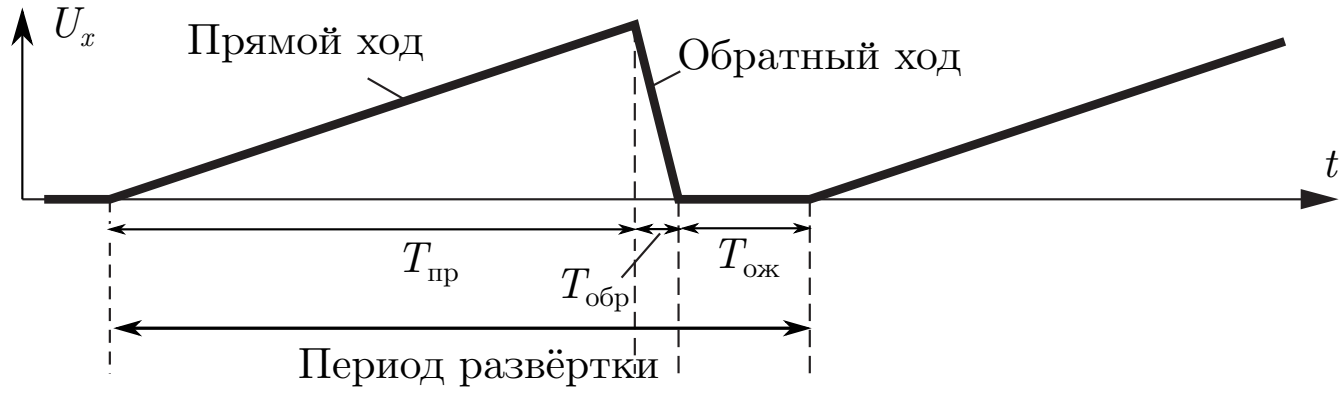
\includegraphics[width=0.5\textwidth]{3.png}
\caption{Напряжение развертки}
\end{wrapfigure}

Для получения на экране «изображения» некоторого электрического сигнала U(t) сам сигнал нужно подать на вертикальные пластины. Подаваемое на вертикально отклоняющие пластины напряжение должно быть пропорционально самому сигналу:  
\[ U_y(t) = U_{0y}+K_{y}U(t)\]
$U_{0y}$ - постоянное напряжение, определяющие расположение графика сигнала по оси $Y$; $K_{y}$ - коэффициент входного сигнала каналом вертикального отклонения.

Подаваемое на горизонтально отклоняющие пластины напряжение должно линейно зависить от времени : 
\[U_x = U_{0x}+ kt\]
$U0y$ и $U0x$ — постоянные напряжения, задающие смещение графика сигнала на экране по осям $Y$ и $X$ соответственно (могут изменяться соответствующими ручками регулировки), $K_{y}$ — коэффициент усиления сигнала по вертикальной оси,; $k$ - коэффициент пропорциональности, зависящий от рабочих харрактеристик генератора развертки и усилителя.

Это напряжение, изображённое на рис. 3, вырабатывает генератор внутренней развёртки осциллографа. В течение времени прямого хода луча напряжение изменяется до максимального значения так, что луч с постоянной скоростью проходит весь экран слева направо. После завершения прямого хода луча начинается процесс обратного хода, когда напряжение развёртки возвращается к первоначальному уровню, а луч переходит в исходное положение в левый край экрана (заметим, что при обратном ходе луча напряжение на модуляторе «запирает» трубку, поэтому свечение экрана не возникает). Скорость изменения напряжения прямого хода развёртки, т. е. масштаб по оси X, задаётся специальной ручкой регулировки, устанавливающей соотношение между временем и числом делений экрана («ВРЕМЯ/ДЕЛ» или «TIME/DIV»). После возврата луч может стартовать не сразу, а находиться в покое в течение времени ожидания, что позволяет синхронизировать отрисовку сигнала (см. ниже). После того, как луч в процессе развёртки дойдёт до края экрана, развёртка должна быть запущена заново. В результате напряжение на горизонтальных пластинах будет иметь пилообразную форму. 

Напряжение пилообразной формы, вырабатываемое генератором развёртки осциллографом, изображено на рисунке. Во время прямого хода луч проходить через весь экран слева направо, после чего напряжение сбрасывается во время обратного хода. Далее после времени ожидания снова появляется луч на экране. Общее время ожидания и обратного хода называется временем блокировки.

При наблюдении периодических быстропротекающих процессов важно зафиксировать изображение на экране, для чего используется синхронизация: для неподвижного изображения необходимо, чтобы период развёртки был кратен периоду излучаемого сигнала, что можно сделать, "навязав" свой период генератору развёртки (для генератора развёртки есть несколько режимов на осциллографе).

\begin{wrapfigure}{R}{.5\textwidth}
\centering
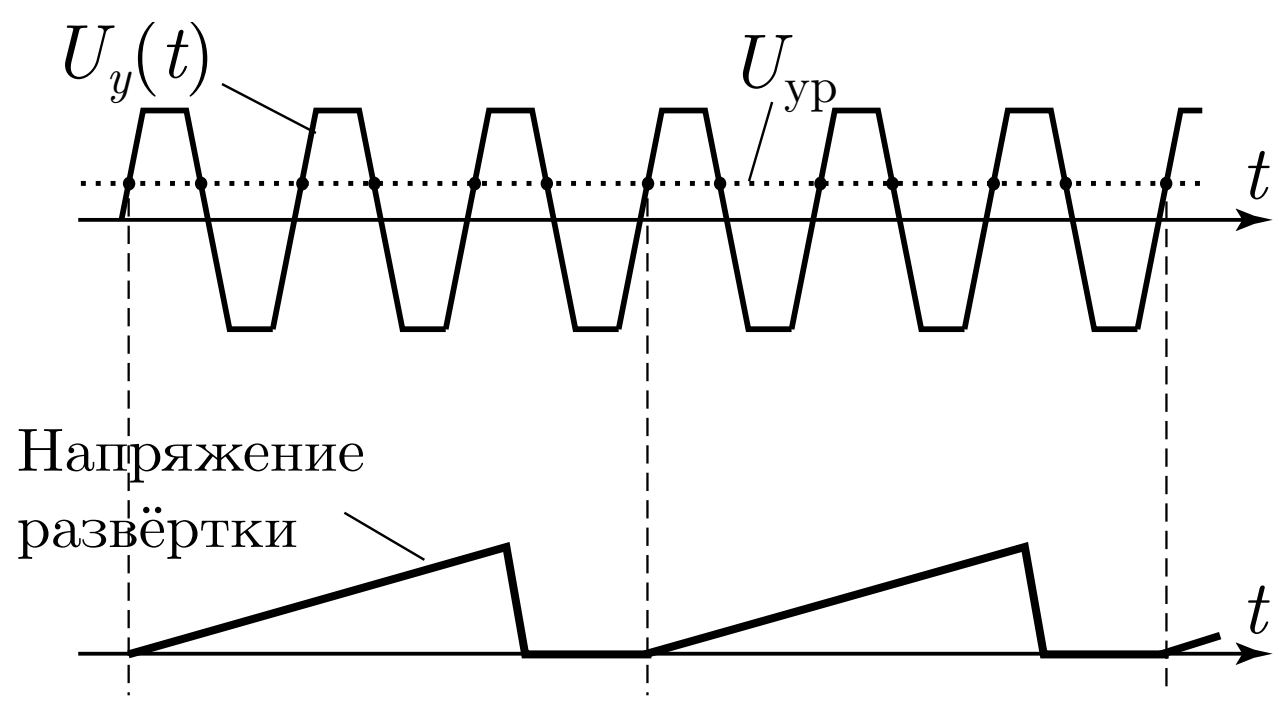
\includegraphics[width=0.4\textwidth]{4.png}
\caption{Синхронизация развертки по заданному уровню}
\end{wrapfigure}

Наиболее часто используется способ синхронизации развёртки по
уровню сигнала. Он поясняется осциллограммами на рис. 4. Периодический сигнал произвольной формы $U_{y}$ сравнивается с некоторым пороговым напряжением $U_{ур}$ — уровнем синхронизации (устанавливается ручкой «УРОВЕНЬ» или «LEVEL» блока управления синхронизацией). После попадания в режим ожидания, прямая развёртка не запускается до тех пор, пока величина сигнала $U_{y}$ не достигнет порогового значения $U_{ур}$, то есть пока не произойдёт пересечение уровня (сверху вниз или снизу вверх, в зависимости от настроек). Таким образом, регулировка уровня синхронизации
позволяет выбрать фазу сигнала в начале развёртки — исходя из наилучшей устойчивости синхронизации и удобства наблюдения. Если $U_{y}$ не пересекает уровень $U_{ур}$, то синхронизация оказывается невозможна.

Осциллограф можно рассматривать как колебательную систему, отклонение которой возбуждается внешним источником. Как у любой колебательной системы, у осциллографа есть амплитудно-частная
(АЧХ) и фазо-частотная (ФЧХ) характеристики. В рабочем режиме отклонение луча на экране осциллографа прямо пропорционально
приложенному напряжению, а задержки в фазе сигнала не возникает.
Однако при приближении к границам полосы пропускания (см. выше),
и тем более при выходе за неё, амплитуда и фаза сигнала на экране
окажется отличающейся от ожидаемой.

Пусть на вход "Y" осциллографа подан гармонический сигнал $U_{y} = U_{0} \cdot sin(2\pi \nu t)$. После "обработки" сигнала осциллографом на его экране будет изображена некоторая зависимость, которая, вообще говоря, может отличаться от исходной: у неё может оказаться другая амплитуда и другая фаза (частота, как правило, сохраняется с хорошей точностью): $y = y_{0} \cdot sin(2\pi\nu t + \varphi)$. Причем амплитуда $y_{0}(\nu)$ и фаза $\varphi(\nu)$ зависят от частоты сигнала $\nu$. Амплитудо-частотной характеристикой (АЧХ) называют отношение:
\[K(\nu) = \frac{y_{0}(\nu)}{U_{0}}\]
В «рабочем» режиме АЧХ постоянна $K(\nu) = const$, а в общем случае АЧХ является функцией частоты сигнала. Фазо-частотной характеристикой (ФЧХ) называют зависящую от частоты величину сдвига фаз $\varphi(\nu)$. ФЧХ осциллографа в рабочем диапазоне частот - это некоторая константа (в идеале - ноль). АЧХ и ФЧХ канала горизонтального отклонения определяются аналогично.

Входные каналы осциллографа могут работать в закрытом (маркируется как $\sim$ или AC) и открытом режиме ($\simeq$ или DC). В закрытом режиме ко входу последовательно подключается разделительный конденсатор, который убирает постоянную составляющую сигнала (конденсатор не пропускает постоянный ток), а на усилитель осциллографа подаётся только переменная составляющая $U_{\sim}$. В открытом режиме подаётся как постоянная, так и переменная составляющие сигнала $U = U_{=} + U_{\sim}$.\par 
В закрытом режиме конденсатор не только не пропускает постоянную составляющую, но и сильно искажает любую медленно меняющуюся (низкочастотную) зависимость — из-за процесса зарядки/разрядки разделительного конденсатора. В связи с этим, низкочастоные АЧХ и ФЧХ закрытого входа могут существенно отличаться
от постоянных.\par
Заметим, что в любом режиме осциллограф обладает большим входным сопротивлением (обычно, 1 МОм), что позволяет считать осциллограф практически идеальным вольтметром — ток через осциллограф мал и, следовательно, его наличие не искажает распределение токов в цепи.

\begin{wrapfigure}{R}{.5\textwidth}
\centering
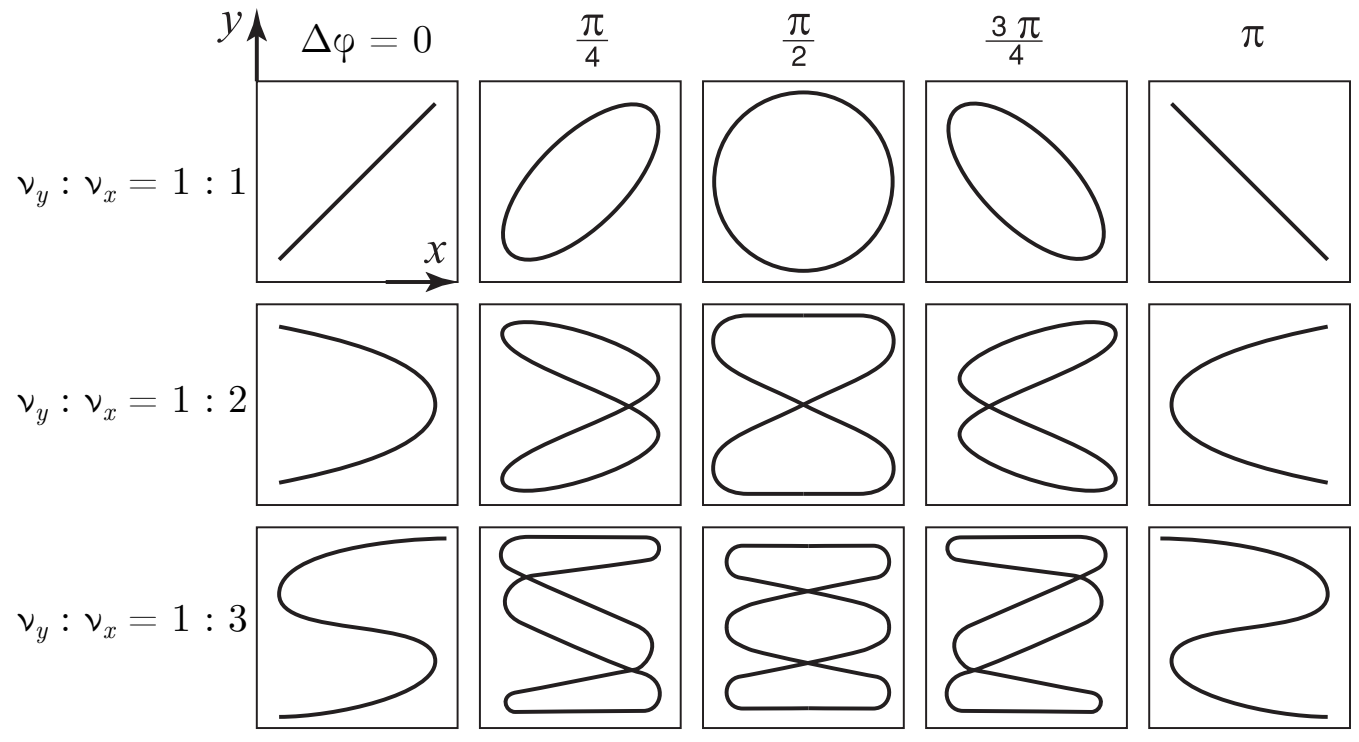
\includegraphics[width=0.55\textwidth]{5.png}
\caption{Фигуры Лиссажу}
\end{wrapfigure}

Помимо наблюдение развёртки сигналов, в любом осциллографе предусмотрен режим совместной подачи двух сигналов $U_{y}(t)$ и $U_{x}(t)$ на вертикальные и горизонтальные отклоняющие пластины (режим «X–Y»). В результате на экране будет наблюдаться результат сложения двух взаимно перпендикулярных колебаний.

Если сигналы:
\[U_{y}(t) = U_{0y}sin(2\pi\nu_{y}t + \varphi_{y})\]
\[U_{x}(t) = U_{0x}sin(2\pi\nu_{x}t + \varphi_{x})\]

являются периодическими с совпадающими или кратными частотами, на экране возникают неподвижные замкнутые кривые, называемые фигурами Лиссажу. Вид фигуры Лиссажу зависит от соотношений между периодами (частотами), фазами и амплитудами складываемых колебаний. Некоторые частные случаи фигур Лиссажу для разных периодов и фаз показаны на рис. 5. При небольшом нарушении кратности частот форма фигур медленно меняется (кажется, что фигуры «вращаются»), а при большом — картина размывается.

При совпадении двух частот $(\nu_{x} = \nu_{y})$ фигура Лиссажу является эллипсом. По форме и ориентации эллипса можно измерить разность фаз между двумя колебаниями. Остановимся на этом вопросе подробнее. 

Рассмотрим два взаимно перпендикулярных колебания одинаковой частоты, но с разными фазами и амплитудами:
\[x = Acos(2\pi\nu t + \varphi_{x}), y = Bcos(2\pi\nu t + \varphi{y}).\]
Исключим из этих уравнений время $t$. После некоторых преобразований с использованием стандартных тригонометрических тождеств можно получить уравнение траектории движения луча на экране:
\[\frac{x^2}{A^2} + \frac{y^2}{B^2} - 2\frac{xy}{AB}cos(\Delta\varphi) = sin^2(\Delta\varphi),\Delta\varphi = \varphi_{y} - \varphi_{x}\]
Таким образом, фигура, которую описывает луч при сложении колебаний одинаковой частоту, представляет собой эллипс. В частных случаях эллипс может «вырождаться» в окружность (A = B, $\Delta\varphi = \frac{\pi}{2}$) или в прямую линию ($\Delta\varphi = 0$).

Если одно или оба колебания происходят не по гармоническому, а по более сложному периодическому закону, то получаются замкнутые траектории более сложной формы.

\section{Ход работы}


\end{document}
